\section{Low Rank}
\label{sec:LowRank}


\subsection{Upright orientation}
\label{subsec:upright orientation}

Most man-made models can be posed at a unique upright orientation which is consistent to human sense. Given a 3D digital model, finding its upright orientation and posing it at the right orientation is vital for users to recognize it.

\begin{figure*}[ht]
  \centering
  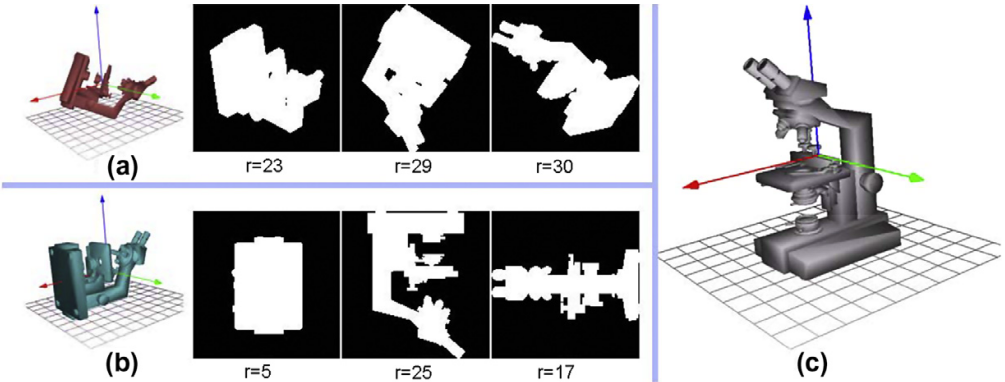
\includegraphics[width=5in]{images/lowrank}
  \caption{Low rank: observation. (a): local method\cite{jin2012unsupervised}. (b): global method\cite{wang2014upright}.}
  \label{fig:lowrank}
\end{figure*}

Figure~\ref{fig:lowrank} shows the axis-aligned projections of an input man-made model with arbitrary(a) and axis-aligned orientation(b) onto the $y$-$z$, $y$-$z$ and $y$-$z$ plane(left to right) in the $x$-$y$-$z$(red-green-blue) coordinate system.
Regarding these projections as two-domensional matrices,
it is clear that the ranks of projection matrices in (b) are significantly $lower$ than those in (a).
And, the upright orientation(c) should be one of the six orientations determined by the six axis-aligned candidate bases, i.e., top, bottom, left, right, front and back surface of the bounding box of the model.
Briefly, ranks of projection matrices at axis-aligned orientations are lower than their counterparts at other orientations, since man-made models are mainly composed by horizonal and vertical edges and shapes.

\paragraph{(1)}
Based on this observation, \cite{jin2012unsupervised} presents an unsupervised approach for finding the upright orientation of man-made models.
Taking the $x$-$y$ plane projection as an example, they binarize the projection as black and white to generate the projection image $I$ with fixed resolution which can also be referred as a two-dimensional matrix.
To avoid affect of noise, $I$ is modeled as a low-rank version $L$ with sparse-error matrix $E$: $I=L+E$.
Then the problem is formulated as

\small{
\begin{equation}
 \label{eq:UprightJin}
 \min_{L,E,R}\|L\|_{*}+\lambda\|E\|_{1},~s.t.~I\circ R=L+E
\end{equation}
}
\\
where $\|\cdot\|_{*}$ and $\|\cdot\|_1$ are the nuclear norm and the $L_1$ norm,
which are closely related to rank and sparsity of matrix respectively.
$R$ is a rigid rotation transformation matrix used to rectify $I$ to recover the optimal low-rank representation of $x$-$y$ plane projection from an arbitrary orientation.

For the whole algorithm, after selecting which projection should be rectified from $y$-$z$, $y$-$z$ and $y$-$z$,
using~(\ref{eq:UprightJin}) the man-made model will be aligned with some axes followed by final upright orientation selection from six orientations as mentioned above.
However, whether a model fits for this algorithm depends on if the model contains dominant parts parallel to the supporting base,
then it will fail if the model is composed by several equivalently main parts which have their own low-rank observation in different orientations.%This method can achieve great result when the model has perfect symmetries.

\paragraph{(2)}It is very natural to generalize this method in 3D space to construct three-order tensor(multidimensional array) with volume of the 3D model, i.e., the three-order tensor ought to have a $"$low rank$"$ behavior. \cite{wang2014upright} constructs this three-order tensor using the bounding box of the 3D model since the bounding box parallels the coordinate planes and contains the whole model. By translating the barycenter of the input model to the origin of the coordinate system, they just need to find and optimal rotation matrix $R$ to align the model with three axes by following optimization model

\small{
\begin{equation}
 \label{eq:UprightJin}
 R_{*}=\mathop{\argmin}_{R}(\|\chi(V\circ R)\|_{*})
\end{equation}
}
\\
where $V$ and $V\circ R$ respectively indicate the point coordinates of input model and the rotated model, $\chi(\cdot)$ is the three-order tensor. Similar to \cite{jin2012unsupervised}, after aligning the model with three axes, they select the upright orientation from six orientations by analyzing the geometric properties.
%
%But when a model has not any external symmetry or the symmetry in a big part whose rank plays the leading role in the low-rank optimization is in consistent with the model, the method may fail as well as \cite{jin2012unsupervised}.
Figure~\ref{fig:upright_lowrank} shows the results of these two methods.

\begin{figure}[ht]
  \centering
  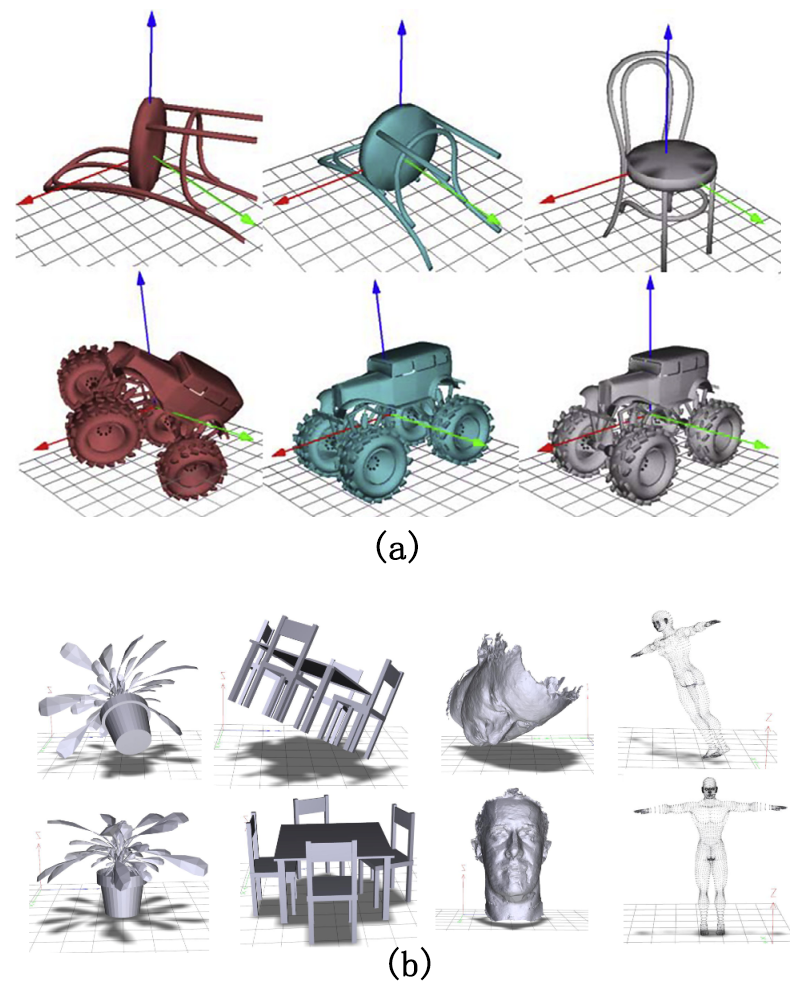
\includegraphics[width=2.5in]{images/upright_lowrank}
  \caption{Low rank: unsupervised upright orientation. (a): local method\cite{jin2012unsupervised}. (b): global method\cite{wang2014upright}.}
  \label{fig:upright_lowrank}
\end{figure}




\subsection{Point cloud normal estimation}
\label{subsec:normal estimation}

Now after reviewing almost all the sparsity based geometric problems, it is clear to us that good normal estimation from noisy data has been always focused since it induces better geometry processing results, like reconstruction, rendering.

Considering that, the neighborhood of a point in a smooth region can be well approximated by a plane, it is easy to get a robust normal estimation.
Thus using the robust results in smooth regions as prior knowledge, \cite{zhang2013point} estimates the point normals around the sharp regions by low-rank clustering(LRSCPK).

In section~\ref{subsubsec:co-segmentation}, we have given an overview about sparse subspace clustering. Low-rank subspace clustering, for capturing the global structure of the whole data, is a modification as

\small{
\begin{equation}
 \label{eq:LSC}
 \min \|Z\|_{*},~\textrm{s.t.}~X=XZ
\end{equation}
}

With an input noisy point cloud $ \mathcal{P}=\{ p_{i} \} {_{i=1}^{N}} $,
they firstly detect the candidate feature points(Figure~\ref{fig:normal_lowrank}(b)) by covariance analysis of the point neighborhoods of size $S$.
Since their neighborhoods are all anisotropic, to segment each neighborhood into several isotropic subneighborhoods,
for each candidate point $p_{i}$, they select a larger neighborhood of size $S^{*}$, i.e., $S^{*}>S$.
In the local coordinates with $p_{i}$ as the origin, the neighbor point $p_{ij}$ of $p_{i}$ is represented as $p_{ij}=[x_{j},y_{j},z_{j},n_{xj},n_{yj},n_{zj}]',j=1,\cdots,S^{*}$,
where $[x_{j},y_{j},z_{j}]$ is the coordinate of $p_{ij}$ and
$[n_{xj},n_{yj},n_{zj}]$ is its normal computed by PCA.
The sampling matrix is defined as $X=[p_{i1},p_{i2},p_{iS^{*}}]$.
The optimal coefficient matrix $Z\in \mathbb{R}^{S^{*}\times S^{*}}$ is computed by solving

\small{
\begin{equation}
 \label{eq:LRSCPK}
 \begin{split}
 & \min \|Z\|_{*} + \beta \| \mathcal{P}_{\Omega}(Z) \|_1
 + \gamma \| E \|_{2,1} ,\\
 &~s.t.~X=XZ+E,
 \end{split}
\end{equation}
}
\\
where, $\Omega,(0\leq\Omega(i,j)\leq1)$, is a guiding matrix constructed according to the distance relation between each two neighbor points for current candidate point. $\mathcal{P}_{\Omega}$ is defined as  $\mathcal{P}_{\Omega}(Z_{i,j})=\Omega(i,j)\times Z(i,j)$.
After getting $Z$, by defining the affinity matrix like section~\ref{subsubsec:co-segmentation}, this larger neighborhood is segmented into several subneighborhoods in which a consistent subneighborhood is used to estimate the current point normal.

\begin{figure}[ht]
  \centering
  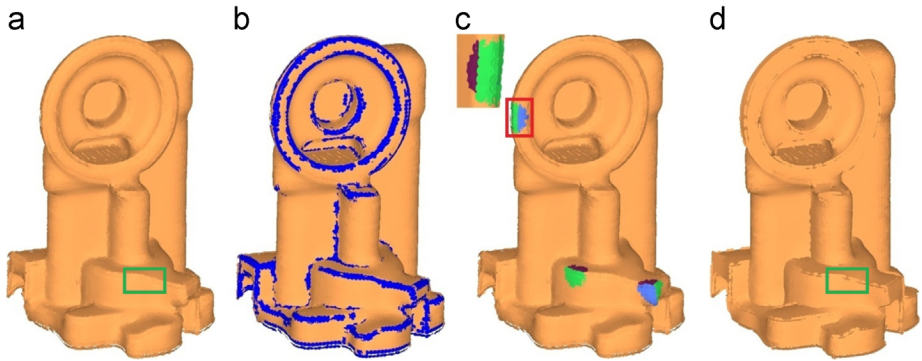
\includegraphics[width=3in]{images/normal_lowrank}
  \caption{Low rank: normal estimation\cite{zhang2013point}. (a): the oil pump module with normal computed by PCA. (b): initial detected candidate feature points. (c): the classified subneighborhoods. The neighborhood within the red box contains three subneighborhoods rendered in blue, green and brown and the zoomed view is from left. (d): estimated normals.}
  \label{fig:normal_lowrank}
\end{figure}
